\section{Method}

\subsection{Overview}

We study cropped vertical single-column ancient-text recognition. Given an input image $x$, the model predicts a character sequence $y=(y_1,\ldots,y_T)$, where $y_t\in\mathcal{A}$ and $\mathcal{A}$ is the target charset. Training primarily uses single-column images and line-level transcriptions. When character boxes are available, SAQT uses them as character-localization supervision, not as a required input at test time.

As shown in Fig.~\ref{fig:overview}, SAQT places detection-style queries between character-localization information and line-level sequence recognition. The framework contains three components: character-localization information learning, charset-aware classifier adaptation, and CTC recognition training. First, character boxes supervise the model to learn character-level visual evidence, character positions, and vertical spatial organization. Second, if the target charset differs from the reference charset associated with the localization-aware query representation, the classifier adaptation module copies parameters for shared characters and initializes parameters for new target characters. Finally, the model is trained with line-level CTC. During recognition, query outputs are sorted by predicted vertical coordinates and decoded as a CTC sequence.

\begin{figure}[t]
  \centering
  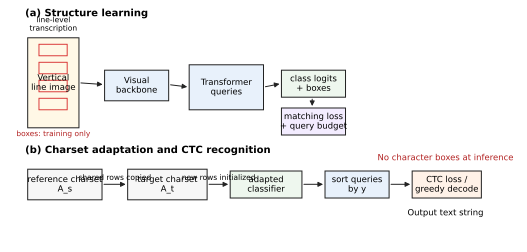
\includegraphics[width=\linewidth]{figures/figure1_saqt_overview.pdf}
  \caption{Overview of SAQT. Character boxes supervise detection-style queries during character-localization information learning, but are not used at inference time. Query outputs are sorted by vertical position and converted into a CTC sequence. Charset-aware classifier adaptation initializes target classifiers when the target charset differs from the reference charset.}
  \label{fig:overview}
\end{figure}

\subsection{Character-Localization Information Learning}

The character-localization information learning stage trains character-aware queries with character-box annotations. For an input image, the model produces $Q$ queries. Each query predicts a character-logit vector $\hat{s}_q\in\mathbb{R}^{|\mathcal{A}_s|}$ and a normalized character box $\hat{b}_q$. Given character annotations $\{(c_i,b_i)\}_{i=1}^{N}$, bipartite matching assigns predicted queries to ground-truth characters or background. The localization objective is
\begin{equation}
\mathcal{L}_{loc} =
\lambda_{cls}\mathcal{L}_{cls}+
\lambda_{box}\mathcal{L}_{box}+
\lambda_{giou}\mathcal{L}_{giou}.
\end{equation}
Here, $\mathcal{L}_{cls}$ supervises query-level character classification, while $\mathcal{L}_{box}$ and $\mathcal{L}_{giou}$ supervise character localization. The box branch is not the final output interface. Instead, its geometry provides the ordering signal needed to convert set-structured queries into an ordered recognition sequence.

A fixed query budget provides enough capacity for long columns, but short columns may produce excessive nonblank activations. We therefore introduce a length-aware query activation budget. For sample $i$, the nonblank activation of query $q$ and the expected number of active queries are
\begin{equation}
a_{i,q}=\max_c\sigma(\hat{s}_{i,q,c}),\qquad
\hat{n}_i=\sum_{q=1}^{Q}a_{i,q}.
\end{equation}
The budget is determined by transcription length $T_i$:
\begin{equation}
n_i^*=\alpha T_i+m,
\end{equation}
where $m$ keeps extra capacity for uncertain alignments. The regularizer penalizes only activations above the budget:
\begin{equation}
\mathcal{L}_{qb}=\frac{1}{B}\sum_i
\frac{\max(0,\hat{n}_i-n_i^*)^2}{\max(T_i,1)}.
\end{equation}
The full localization-aware query learning loss is
\begin{equation}
\mathcal{L}_{clq}=\mathcal{L}_{loc}+\lambda_{qb}\mathcal{L}_{qb}.
\end{equation}
The constraint is one-sided: it suppresses excessive nonblank activations, but it does not force every sample to use a fixed number of queries. Transcription length is used only during training.

\subsection{Charset-Aware Classifier Adaptation}

If the target charset is identical to the reference charset, SAQT can reuse the original classifier or train a classifier from scratch. If the charsets differ, SAQT applies charset-aware classifier adaptation. Let $\mathcal{A}_s$ and $\mathcal{A}_t$ denote the reference and target charsets. For shared characters, the target classifier inherits the corresponding reference parameters:
\begin{equation}
W_t[i]=W_s[j],\quad b_t[i]=b_s[j],
\quad \text{if } \mathcal{A}_t[i]=\mathcal{A}_s[j].
\end{equation}
For target characters absent from the reference charset, the target rows are initialized from unused reference classifier rows when available; if not enough rows are available, reference rows are randomly reused:
\begin{equation}
W_t[i], b_t[i]\leftarrow W_s[k], b_s[k],
\quad \text{if } \mathcal{A}_t[i]\notin\mathcal{A}_s.
\end{equation}
This adaptation is applied to the decoder classification heads and the encoder output classification head. After adaptation, we first train the reconstructed heads to align the target classifier with the localization-aware query representation, and then continue full-model recognition training. This module is a training initialization strategy rather than an inference-time component.

\subsection{CTC Recognition Training and Decoding}

During recognition training, the model is trained with target line-level transcriptions. CTC requires an ordered probability sequence, whereas query outputs are set-structured. SAQT sorts queries from top to bottom using predicted vertical box coordinates, converts sorted logits into token probabilities with an explicit blank class, and inserts blank-only positions between neighboring query positions. Low-confidence queries allocate remaining probability mass to blank; high-confidence nonblank queries keep a small blank floor and renormalize nonblank probabilities.

Given the resulting probability sequence $p_1,\ldots,p_U$, the CTC objective is
\begin{equation}
\mathcal{L}_{ctc}=
-\log
\sum_{\pi\in\mathcal{B}^{-1}(y)}
\prod_{u=1}^{U}p_u(\pi_u),
\end{equation}
where $\mathcal{B}$ merges repeated tokens and removes blanks. This formulation links character-localization information with sequence recognition while requiring only line-level transcriptions downstream.

To reduce mismatch between the expected number of nonblank CTC positions and the transcription length, we further use a lightweight optional length-consistency auxiliary term. Let $p_{u,c}$ be the probability that the $u$-th sorted CTC position predicts character $c$. The expected number of nonblank positions is
\begin{equation}
\hat{T}=\sum_{u=1}^{U}\sum_{c\neq\varnothing}p_{u,c}.
\end{equation}
Given transcription length $T$, the auxiliary term constrains the ratio between the expected nonblank count and the ground-truth length:
\begin{equation}
\mathcal{L}_{cnt}=
\operatorname{SmoothL1}
\left(
\frac{\hat{T}}{\max(T,1)}, 1
\right).
\end{equation}
For very short columns, this term can be assigned a higher weight to reduce deletion caused by overly dominant blank predictions. It does not change the model structure or inference pipeline, and we treat it as a lightweight optional auxiliary module rather than the sole core design of SAQT.

At inference time, greedy CTC decoding can be sensitive to the relative confidence of blank and nonblank tokens. We therefore use a lightweight logit calibration:
\begin{equation}
\tilde{z}_{u,\varnothing}=z_{u,\varnothing}+\beta_b,\qquad
\tilde{z}_{u,c}=z_{u,c}+\beta_{nb},\; c\neq\varnothing,
\end{equation}
where $\varnothing$ denotes blank. The bias pair $(\beta_b,\beta_{nb})$ is determined by a development-set calibration protocol and then fixed for testing. This step uses no language model or external text data.
